\documentclass[lettersize,journal]{IEEEtran}
\usepackage{amsmath,amsfonts}
\usepackage{algorithmic}
\usepackage{algorithm}
\usepackage{array}
\usepackage[caption=false,font=normalsize,labelfont=sf,textfont=sf]{subfig}
\usepackage{textcomp}
\usepackage{stfloats}
\usepackage{url}
\usepackage{verbatim}
\usepackage{graphicx}
\usepackage{cite}
\usepackage{tabularx}
\usepackage{boldline}
%\usepackage[justification=centering]{caption}
%\usepackage{hyperref}
\hyphenation{op-tical net-works semi-conduc-tor IEEE-Xplore}
% updated with editorial comments 8/9/2021

\makeatletter
\def\endthebibliography{%
	\def\@noitemerr{\@latex@warning{Empty `thebibliography' environment}}%
	\endlist
}
\makeatother


\begin{document}

\title{Raiden. Power System Transient Stability Simulation Software Prototype}

\author {Eugene Mashalov, Joint Stock Company "Scientific and Technical Center of Unified Power System", Ekaterinburg, Russia}


%\markboth{Journal of \LaTeX\ Class Files,~Vol.~14, No.~8, August~2021}%
%${Shell \MakeLowercase{\textit{et al.}}: A Sample Article Using IEEEtran.cls for IEEE Journals}

%\IEEEpubid{0000--0000/00\$00.00~\copyright~2021 IEEE}
% Remember, if you use this you must call \IEEEpubidadjcol in the second
% column for its text to clear the IEEEpubid mark.

\maketitle

\begin{abstract}
This paper discusses implementation details of the transient stability analysis prototype software based on the implicit integration scheme. The main advantages of an implicit integration scheme with separate treatment of differential and algebraic state variables as well as an integration process with discrete event handling are considered. The results of test simulations and their comparison with existing software packages are presented.
\end{abstract}

\begin{IEEEkeywords}
Transient Stability Analysis, Implicit Integration, Discontinuous DAE
\end{IEEEkeywords}

\section{Introduction}
\IEEEPARstart{T}{ransient} stability simulation is one of the most complicated tasks of power system analysis. Besides methodological complexity, it requires intense computation with significant time consumption. Parallel implementation of simulation algorithms is difficult due to the sequential nature of the solution method, which is based on integration of the differential-algebraic system of equations (DAE), which is hardly separable into weakly connected parts. Thus, even modern computer systems do not provide the opportunity for real-time simulation, unless model details are reduced. Transient stability is dominantly used in offline applications, such as facility development, and rarely used for power system control on a time scale close to real-time.

However, some near-real-time implementations have been introduced in the last decade. One of the most successful is the stability monitoring system, used by the System Operator of Russia. The system evaluates the safe limits of network load over a period of 40–900 s with respect to static and transient stability. However, some near-real-time implementations have been introduced in the last decade. One of the most successful is the stability monitoring system, used by the System Operator of Russia. The system evaluates the safe margins of network load over a period of 40–900 s with respect to static and transient stability. These margins are used for system automatic or manual control. The duration of the evaluation cycle is mostly determined by the duration of the transient stability simulation. The aim of reducing the computation time of simulation led to the development of the software prototype based on the implicit integration scheme, instead of the former implementation based on explicit methods. The new algorithm consists of three components of integration: the method, the scheme, and the process. However, some near-real-time implementations have been introduced in the last decade. One of the most successful is the stability monitoring system, used by the System Operator of Russia. The system evaluates the safe margins of network load over a period of 40–900 s with respect to static and transient stability. These margins are used for system automatic or manual control. The duration of the evaluation cycle is mostly determined by the duration of the transient stability simulation. The aim of reducing the computation time of simulation led to the development of the software prototype based on the implicit integration scheme, instead of the former implementation based on explicit methods. The new algorithm consists of three components of integration: the method, the scheme, and the process. The integration method defines the numerical properties of the problem solution. The integration scheme defines the computation process of the method to ensure optimal utilization of the problem properties. And finally, the integration process arranges the operation of the integration scheme, considering discrete events and discontinuities in the model.

\section{Transient stability simulation algorithm development}
Time spent on transient simulation is proportional to the number of numerical integration steps of the system \eqref{eqn_thedae}: 

\begin{equation}
	\label{eqn_thedae}
	\begin{array}{c}
		\begin{cases}
			\begin{array}{lcl}
				\dot{y}&=&f(x(t), y(t), t) \\
			 	      0&=&g(x(t), t(t), t)\\
			\end{array}
		\end{cases} 
	\vspace{0.5em} \\
	 x(t_0)=x_0, y(t_0)=y_0 \\
	\end{array}
\end{equation}
\noindent where \(g\) and \(f\) are smooth vector functions. The time of simulation initialization and computation of the initial conditions is much smaller than the time of the \eqref{eqn_thedae} solution. The latter depends on the integration method properties and the system dimension \(N_e\). As a rule, solution time \(T_{hn}=O(N_e^3)\), since the integration step in one form or another requires the solution of a system of nonlinear algebraic equations. The value of the integration step \(h_n\) is determined by the properties of the DAE. The crucial property of \eqref{eqn_thedae} with respect to \(h_n\) is the stiffness of the DAE, estimated as the ratio of the maximum and minimum values of the real part of the eigenvalues of its linearized matrix. 

\subsection{The integration method}

In most cases, the transient stability problem \eqref{eqn_thedae} is considered stiff, which encourages using implicit integration methods for its solution. The integration method is a vector function \(F(x,y)\) which maps values from the previous step \(y_{n-1}\) to current step values \(y_n\). Of course, the current step values of \(x_{n} \leftarrow x_{n-1}\) are also required, but there are several approaches to performing this. The general form of the implicit method for differential variables is:
\begin{equation}
	\label{eqn_implicit}
	F(y_n,y_{n-1},t)=0
\end{equation}

The solution of (3) involves the solution of the nonlinear system of equations, which is associated with some technical complications. That was the main reason for the former implementation of transient stability software, which was developed in the 1980s relying on explicit methods. The solution of \eqref{eqn_implicit} implies the solution of the nonlinear system of equations, which is associated with some technical complications. Integration step control bounds solution to:

\begin{equation}
	\label{eqn_z}
	\begin{array}{c}
		\vert\vert z(t_n)-z_n(t_n) \vert\vert <= \epsilon, \\
		z_n(t_n)=[y_n(t_n), x_n(t_n)]^T	 \\
		z(t)=[y(t), x(t)]^T \\
	\end{array}
\end{equation}
\noindent where
\begin{description}
	\item  \(z_n(t_n)\) is the approximated solution;
	\item  \(z(t)\) is the exact solution;
	\item  \(\epsilon\) is the error tolerance;
\end{description}

The step control allows one to vary \(h_{n}=t_{n}-t_{n-1}\) according to \eqref{eqn_z}. For transient phases with rapid changes, the step is reduced. When the transient decays, the step can be increased, which significantly reduces the number of steps required to solve \eqref{eqn_thedae}.

The implicit method implementation is much more complicated than the explicit one, as it requires a non-linear system of equations solution. In most cases, this solution is provided by the Newton method. Power system equipment models should be implemented with respect to this requirement and provide the ability to construct blocks of partial derivatives of the Jacobi matrix. The use of the automatic implementation system can overcome this problem \cite{mycompiler}. Another problem that arises from nonlinearities is the possibility of multiple solutions at the time instants of discontinuities. However, the problems where \eqref{eqn_thedae} has discontinuous \(f\) and \(g\) are well known and there are various approaches developed. Some use rigorous discontinuity modeling \cite{Filippov1988}, while others use integration restart techniques \cite{cellier06}.

\subsection{The integration scheme}

The DAE \eqref{eqn_thedae} solution implies discretization into a pure algebraic system of equations using a chosen integration method. Since the resulting system is nonlinear, an iterative solution method is used. The simplest method is fixed point iteration. This method is usable, but, in many cases, does not provide convergence due to its limitations. The application of the Newton method requires Jacobian matrix formation, which greatly increases the equipment models development complexity. In addition to the system of equations for each model, it is also required to form a block of the Jacobi matrix. However, Newton's method makes it possible to reliably obtain a solution, has good convergence, and, moreover, can be used not only to solve \eqref{eqn_thedae} but also to determine the initial conditions at \(t=0\) and at the time points of discrete changes \(t_d\). The weak side of Newton's method is its sensitivity to the quality of the initial guess. This problem is partly solved by using the initial estimation from the previous integration step. An additional factor that improves the convergence of Newton's method can be the scheme of the integration method. A well-known integration approach is the predictor-corrector scheme. With values of the available solution \(z_{n-1}\) at the time \(t_{n-1}\), the method can predict the values of \(z_n\) using extrapolation. The resulting prediction is used as an initial estimation for solving the equivalent \eqref{eqn_thedae} system, in which the differential equations are discretized in a form that depends on the chosen integration method. During the solution, the prediction is corrected so that the values satisfy the given system of equations. This scheme is effectively implemented using multi-step integration methods, which imply saving the data of several completed steps to perform the next step. To solve DAE, this approach is implemented in the Gear method \cite{gear71}. This method involves the use of the BDF integration method, both for differential and algebraic equations, and provides a simultaneous solution to \eqref{eqn_thedae}. Such an integration scheme is fully implicit and preserves integration method stability properties.

A variant of the Gear method is implemented in the well-known software EUROSTAG \cite{mixedadams}. Since the methods of the BDF family have the property of damping high-frequency oscillations with an increase in the integration step, the Gear method exhibits "hyperstability" and erroneously treats unstable cases as stable. The proposed modification, which consists of applying the Adams method for differential variables, eliminates this drawback. A variant of the Gear method is implemented in the well-known software Eurostag [8]. Since the methods of the BDF family have the property of damping high-frequency oscillations with an increase in the integration step, the Gear method exhibits hyperstability and erroneously treats unstable cases as stable. The proposed modification, which consists of applying the Adams method to differential variables, eliminates this drawback since the 2nd order Adams method is A-stable. The use of the BDF for algebraic variables makes it possible to maintain a higher integration step compared to the Adams method with the same overall stability properties of the integration scheme.

All linear multistep methods of order \(q\), despite significant differences in their properties, can be expressed in Nordsieck form \cite{hairer93}. That vector has a dimension of \(1 \times q+1\). Since the integration method must be A-stable order is constrained \((q<=2)\) and the maximum dimension of the Nordsieck vector is fixed at \(1 \times 3\). 

At the n-th integration step, Nordsieck vector components of differential and algebraic variables are:
\begin{equation}
	\label{eqn_nords}
	\begin{array}{cc}
		Y_n=\left[y_n, h_n \dot{y}_n, \frac{h_n^2}{2} \ddot{y}\right], &
		X_n=\left[x_n, h_n \dot{x}_n, \frac{h_n^2}{2} \ddot{x}\right] 
	\end{array}
\end{equation}

The Nordsieck vector is merely a form to express the Taylor's expansion of \(x_n\) and \(y_n\) at \(t_n\). If this vector for \(t_{n-1}\) is known, the prediction at \(t_n\) is:

\begin{equation}
	\label{eqn_predictor}
	\begin{array}{cc}
		Y_n^0=Y_{n-1}A, &
		X_n^0=X_{n-1}A
	\end{array}
\end{equation}

\noindent where 
\begin{description}
	\item  \(Y_n^0\) is the differential variables vector extrapolated to \(t_n\);
	\item  \(X_n^0\) is the algebraic variables vector extrapolated to \(t_n\);
	\item  \(A\) is the lower triangular Pascal matrix \(q+1 \times q+1\).
\end{description}

The corrected Nordsieck vector at \(t_n\) is: 
\begin{equation}
	\label{eqn_corrector}
	\begin{array}{cc}
		Y_n=Y_n^0 +l^Ye_{yn}, &
		X_n=X_n^0 +l^Xe_{xn},
	\end{array}
\end{equation}
\noindent where 
\begin{description}
	\item  \(l^Y\) is the row vector of integration method for differential variables;
	\item  \(l^X\) is the row vector of integration method for algebraic variables;
	\item  \(e_{yn}, e_{xn}\) are the error vectors with respect to the predicted vectors;
\end{description}
The vectors \(e_{yn}, e_{xn}\) are normalized:
\begin{equation}
	\label{eqn_nordnormal}
		l^Y_1=l^X_1=1
\end{equation}
The corrector equations \eqref{eqn_corrector} can be written by components:
\begin{equation}
	\label{eqn_corrcomp}
	\def\arraystretch{1.4}
	\begin{array}{l}
		\begin{array}{rllll}
			y_n &= &y_n^0&+&l_0^Ye_{yn} \\
			h_n \dot{y}_n &=& h_n \dot{y}_n^0&+&l_1^Ye_{yn} \\
			\frac{h_n^2}{2}\ddot{y}_n &=& \frac{h_n^2}{2}\ddot{y}_n^0& + &l_2^Ye_{yn}
		\end{array}
		\\
		\begin{array}{rllll}
			x_n &= &x_n^0&+&l_0^Xe_{xn} \\
			h_n \dot{x}_n &=& h_n \dot{x}_n^0&+&l_1^Xe_{xn} \\
			\frac{h_n^2}{2}\ddot{x}_n &=& \frac{h_n^2}{2}\ddot{x}_n^0& + &l_2^Xe_{xn}
		\end{array}
	\end{array}
\end{equation}

From the \(\dot{y}_n\) equation from \eqref{eqn_corrcomp}:
\begin{equation}
	\label{eqn_corrdiff}
	\def\arraystretch{1.1}
	\begin{array}{l}
		h_n\dot{y}_n =  h_nf(x_n,y_n,t_n)\\
		h_n\dot{y}_n^0+l_1^Ye_{yn} - h_nf(x_n,y_n,t_n) = 0
	\end{array}
\end{equation}
Using \eqref{eqn_nordnormal} define:
\begin{equation}
	\label{eqn_define}
	\begin{array}{c}
		F_Y(e_{xn}, e_{yn}, t) = h_n\dot{y}_n^0+e_{yn}-h_nf(x_n, y_n, t_n) \\
		F_X(e_{xn}, e_{yn}, t) = g(x_n, y_n^0+l_0^Ye_{yn}, t_n)
	\end{array}
\end{equation}

\noindent from which the following system can be obtained:
\begin{equation}
	\label{eqn_system1}
	\begin{array}{c}
		\begin{cases}
			\begin{array}{rcl}
			F_Y(e_{xn}, e_{yn}, t) &=&0 \\
			F_X(e_{xn}, e_{yn}, t) &=&0 
			\end{array}
		\end{cases} 
	\end{array}
\end{equation}
\noindent with Jacobi matrix (\(n\) step index is omitted for simplicity):

\begin{equation}
	\label{eqn_jacobi1}
	J = \begin{bmatrix}
		\frac{\partial F_Y(e_x, e_y, t)}{\partial e_y}  +  \frac{\partial F_Y(e_x, e_y, t)}{\partial e_x} \\
		\frac{\partial F_X(e_x, e_y, t)}{\partial e_y}  +  \frac{\partial F_X(e_x, e_y, t)}{\partial e_x}
	\end{bmatrix}
\end{equation}
The combination of \eqref{eqn_define} and \eqref{eqn_jacobi1} gives:
\begin{equation}
	\label{eqn_jacobi2}
	J = \begin{bmatrix}
		I - h_nl_0^Y\frac{\partial f(x, y, t)}{\partial y}  -  h_nl_0^X\frac{\partial f(x, y, t)}{\partial x} \\
		l_0^Y\frac{\partial g(x, y, t)}{\partial y} +  l_0^X\frac{\partial g(x, y, t)}{\partial x} 
	\end{bmatrix}
\end{equation}
Note that the Jacobi matrix does not become singular with \(h_n\rightarrow 0\), which allows it to be used to solve DAE for initial conditions \(y_d\), \(x_d\) at instants of discontinuities \(t_d\). In addition, step reduction does not cause numerical problems, which, for example, the integration scheme \cite{petzold82} is subject to.

The system of equations \eqref{eqn_system1} can be solved iteratively. Variables at iteration \(m\) are:

\begin{equation}
	\label{eqn_mitervars}
	\begin{array}{c}
		\def\arraystretch{1.3}
		\begin{array}{c}
			\begin{cases}
				\begin{array}{l}
					y_n^m =y_n^0+l_0^Ye_{yn}^m \\
					x_n^m =x_n^0+l_0^Xe_{xn}^m \\
				\end{array} \\
			\end{cases} \\
			e_{xn}^0=e_{yn}^0= 0 
		\end{array}
	\end{array}
\end{equation}

The iterative process of solving \eqref{eqn_system1} with respect to \(e_x\) and \(e_y\) is performed according to the recursive formula (\(n\) step index is omitted for simplicity):
\begin{equation}
	\label{eqn_fulliter1}
	\begin{bmatrix}
		e_{y}^{m+1} \\
		e_{x}^{m+1} 
	\end{bmatrix}
	+ 
	\begin{bmatrix}
		e_{y}^m \\
		e_{x}^m 
	\end{bmatrix}
	+ (J^{m})^{-1}
	+
	B^m
\end{equation}
\noindent where:
\begin{equation}
	B^m = 
	\begin{bmatrix}
		h_nf(x^m, y^m, t) - h \dot{y}^0 - e_y^m \\
		-g(x^m, y^m, t_n) 
	\end{bmatrix}
\end{equation}

\noindent and:

\begin{equation}
	J^m = \begin{bmatrix}
	I - h_nl_0^Y\frac{\partial f(x^m, y^m, t)}{\partial y}  -  h_nl_0^X\frac{\partial f(x^m, y^m, t)}{\partial x} \\
	l_0^Y\frac{\partial g(x^m, y^m, t)}{\partial y} +  l_0^X\frac{\partial g(x^m, y^m, t)}{\partial x} 
\end{bmatrix}
\end{equation}

When the process \eqref{eqn_fulliter1} converges, the Nordsiek vectors \(X_n\) and \(Y_n\) at the \(t_n\) are updated using \eqref{eqn_corrector}.
\subsection{Local truncation error control}
The solution of \eqref{eqn_fulliter1} is the difference between predicted and corrected values of the state variables. It is used for local truncation error estimation. The next integration step and integration method optimal order can be further determined using error estimation. Local truncation error \(d_n\) at the step \(n\):
\begin{equation}
	d_n=C_{q+1}q!l_qe_n
\end{equation}
\noindent where \(C_{q+1}\) is the integration method constant.

Since state variables may have very different magnitudes, it is common to use weighted differences for error estimation:

\begin{equation}
	W_{in}=Rtol_i|Z_{i,n-1}|+Atol_i
\end{equation}
\noindent where:
\begin{description}
	\item \(Atol_i\) is the absolute tolerance of i-th state variable;
	\item \(Rtol_i\) is the relative tolerance of i-th state variable.
\end{description}

The condition \eqref{eqn_dn} is used to accept step \(n\). 
\begin{equation}
	\label{eqn_dn}
	\vert\vert d_n \vert\vert = \sqrt{\frac{1}{N} \sum_{i=1}^{N}{\left(\frac{d_{i,n}}{W_{i,n}}\right)^2}} \leq 1
\end{equation}
\noindent where \(N\) is the number of state variables.
If \eqref{eqn_dn} holds, the step and the order of the integration method are adjusted for the next step. The step is rejected and repeated otherwise with a smaller \(h\).

The choice of the norm type for \(d\) estimation has a strong influence on the quality of the simulation. The default option is \(l^2\)-norm, which is acceptable both for the quality of the solution and step size control. As the \eqref{eqn_thedae} is stiff, differential equations with small time constants tend to produce large differences between predicted and corrected values. The \(l^2\)-norm averages these differences and allows step size to be larger.  However, this averaging property degrades the quality of simulation for models with large dimensions due to the "masking" of unacceptable errors in some state variables. In some cases, these errors have a crucial influence on the stability simulations and may lead to erroneous estimation of unstable cases as stable. Using \(l^\infty\)-norm overcomes this problem but leads to an unacceptable time step decrease. A hybrid norm was proposed in \cite{pegase10}, which combines properties of \(l^2\)- and \(l^\infty\)-norms. In this paper, a similar approach based on the weighting of norms is applied.

The operations of integration step and order change induce extra computation costs and should not be used at every step. Step size and order control are based on the strategy described in \cite{Radhakrishnan1993}, where these aspects are considered in relation to the pure differential system of equations. Since the problem being solved is differential-algebraic and stiff, additional measures for convergence control of the corrector and excessive step change suppression are implemented on the basis of \cite{petzold82}.

\subsection{Adams integration method ringing suppression}

The implicit 2nd-order Adams method, also known as the trapezoidal rule, has the property of "ringing" with the increase of the integration step. Ringing appears as oscillations of state variables at transient decay phases where the integration step is relatively large. Ringing does not affect the quality of simulations considerably, but prevents the growth of the integration step, despite the fact that the physical process tends to a steady state.

The 2nd-order Adams method \eqref{eqn_adams} applied to the model equation \(\dot{y}=\lambda y, y(0)=y_0\) gives expression \eqref{eqn_adamsmodel}.
\begin{equation}
	\label{eqn_adams}
	y_n=y_{n-1}+\frac{h}{2}\left(\dot{y}_{n-1}+\dot{y}_n\right)
\end{equation}
\begin{equation}
	\label{eqn_adamsmodel}
	y_n=y_0 \left( \frac{2+h\lambda }{2-h\lambda } \right)^n
\end{equation}
\begin{equation}
	\label{eqn_adamsinf}
	\lim_{h\rightarrow\infty}{ \left( \frac{2+h \lambda }{2-h \lambda } \right) } = -1
\end{equation}
As the integration step increase the \eqref{eqn_adamsinf} holds, which leads to the state variable sign change \((-1)^n\) at every integration step. To suppress ringing, it is necessary to eliminate the influence of the property \eqref{eqn_adamsinf} to the solution. There are several approaches to this problem. For the chosen integration scheme, good results are obtained by replacing \(\dot{y}_n\) proposed in \cite{Lee2015}, after obtaining the solution \(y_n\) by \eqref{eqn_adams}, by the value \(\dot{y}_n^{BDF}\), computed by \eqref{eqn_adamsdsamp}.

\begin{equation}
	\label{eqn_adamsdsamp}
	\begin{array}{c}
	\dot{y}_n^{BDF}=\frac{\alpha^2y_{n-2}-(1+\alpha)^2y_{n-1}+(1+2\alpha)y_n}{h_n(1+\alpha)} \\
	\alpha=\frac{h_n}{h_{n-1}}
	\end{array}
\end{equation}
At the step \(n+1\) the expression \eqref{eqn_adams} would use \(\dot{y}_n^{BDF}\) instead of the value \(\dot{y}_n\) computed at the step \(n\), as shown in \eqref{eqn_modadams}.

\begin{equation}
	\label{eqn_modadams}
	y_{n+1}=y_n+\frac{h}{2}\left(\dot{y}_n^{BDF}+\dot{y}_{n+1} \right)
\end{equation}

Since replacement \(\dot{y}_n^{BDF} \rightarrow \dot{y}_n\) changes integration method stability properties, it is applied only when ringing is detected. The extra conditions to apply this artificial damping are \(h_n>0.1\) s and a cool-down period of several steps before the next damping. The effect of damping is shown in Fig. \ref{fig_adams_damping_variable} and Fig. \ref{fig_adams_damping_step}.

\begin{figure}[htbp]
	\centering
	
\includegraphics[width=0.8\columnwidth]{adams_damping_variable.eps}
	\caption{The ringing suppression effect of 2nd-order Adams damping on state variable evolutions }
	\label{fig_adams_damping_variable}
\end{figure}

\begin{figure}[htbp]
	\centering
	
\includegraphics[width=0.8\columnwidth]{adams_damping_step.eps}
	\caption{The ringing suppression effect of 2nd-order Adams damping on integration step size evolutions (log scale) }
	\label{fig_adams_damping_step}
\end{figure}

\subsection {The integration process}
The integration method and scheme considered above assume that the \eqref{eqn_thedae} is continuous. When simulating practical transients, this condition is not met since some of the \(f\) and \(g\) are not smooth over their entire domain due to constraints or are discrete. In addition, to simulate discrete events, some of the equations of the system have to be modified. In some cases, the dimension of the system also changes. Problems in which system \eqref{eqn_thedae} is not continuous are the separate problem class for DSAR – Differential Switched Algebraic and State Reset equations \cite{Hiskens01}. An obvious approach for solving such problems is integrating a sequence of continuous DAEs.

The problem of DSAR treatment consists of the arrangement of a transition from one continuous DAE to the next one at a time instant defined with consistent initial conditions. The last problem is not trivial, since the nonlinearity and the presence of discrete functions make multiple solutions possible. Due to the additional information available in the history of solution and specified in the form of rules in the models \cite{mycompiler}, the ambiguity can be resolved by a formal choice of the most plausible combination of state variables.

Thus, a full-fledged algorithm for transient stability simulation should implement the integration process, which governs the integration scheme and solves the following problems:
\begin{enumerate}
	\item Discrete events management.
	\item Discontinuities handling.
	\item Calculation of initial conditions and restart of integration
	\item State events time instants location.
\end{enumerate}

The discrete event is a command to modify \eqref{eqn_thedae} at an arbitrary time instant \(t_d\). Command execution requires at least a restart of the integration. In general, some modifications of \eqref{eqn_thedae} structure are also needed. The new consistent initial conditions at \(t_d\) must be calculated to resume integration.

Discrete events can be divided into two groups: time events and state events \cite{cellier06}.  The events of the first group occur at the moments of time that are known before simulation. These include simulation stop time, application of disturbances or triggered time delays. State events occur when some conditions are met. They are connected with threshold elements, limiters, comparators, relays and so on.  Their time of occurrence must be determined during the simulation. 

Discrete event processing is independent of the group it is related to, if \(t_d\) is known. This instant must be located for state events. Assume integration method steps from \(t_{n-1}\) to \(t_n\) and \(t_{n-1}<t_d<t_n\). Discrete event processing must be handled in the following sequence:
\begin{enumerate}
	\item At \(t_{n-1}\) choose \(h_d=t_d-t_{n-1}\) and step to \(t_d\). Let \(t_n=t_d\).
	\item Estimate local truncation error of the step.If tolerance is violated, reject the step, return to \(t_{n-1}\) and choose a new step size according to the error.
	\item At \(t_d\) store simulation results. Since the discrete event considered instant, the time before the event is denoted by \(t_{d-}\) and the time after the event is \(t_{d+}\). Strictly \(t_{d+}>t_d>t_{d-},  t_{d+}-t_{d-} \rightarrow 0\), but to preserve integration method numerical stability in practice \(t_d=t_{d-} = t_{d+}-0.1h_{min}\), where \(h_min\) the is smallest integration step allowed.
	\item Modify \(f\) and \(g\) according to discrete event and solve system \eqref{eqn_system1} with \(h_n=0\). The latter implies \(y_n=y(t_{d-})=y(t_{d+})=const\). The solution of \eqref{eqn_system1}  by an iterative method may be difficult due to a bad initial guess. Therefore, the linear method is used to improve the initial guess and the Newton scheme uses step control, as opposed to the Newton scheme used for integration step \eqref{eqn_fulliter1}.
	\item In case \eqref{eqn_system1} solved successfully, store simulation results at \(t_{d+}\).
	\item Restart the integration scheme from initial conditions \(x_n, y_n\) obtained from \eqref{eqn_system1} solution. Restart sets the integration method order to 1st and \(h_n=h_{min}\).
\end{enumerate}
Since a state event instant must be located, special zero-crossing functions are used to model the conditions of a state event in the form \eqref{eqn_zcbase}.
\begin{equation}
	\label{eqn_zcbase}
	z_i(t) > Ref_i(t)
\end{equation}
\noindent where \(Ref_i(t)\) is zero-crossing function of the i-th state variable.

Usually zero crossing functions are considered as algebraic equations in \eqref{eqn_thedae} in the form \eqref{eqn_zcindae}.
\begin{equation}
	\label{eqn_zcindae}
	c_j(t)=z_i(t)-Ref_i(t)
\end{equation}
\noindent which sign change \(c_j(t_{d-}) c_j(t_{d+}) < 0 \) indicates \(t_d\) location. This condition can be checked at the final stage of the integration step.
For zero-crossing functions, whose signs have been changed \(t_d \in [t_{n-1}, t_n]\) should be located with accuracy up to \(h_{min}\). Since the integration scheme is based on the multistep integration method at \(t_n\) a Nordsieck vector is available for all state variables (including algebraic ones) up to 2nd order \eqref{eqn_zcnord}.
\begin{equation}
	\label{eqn_zcnord}
	\left[ c_{jn}, h_e\dot{c}_{jn}, \frac{h_e^2}{2}\ddot{c}_{jn}\right]
\end{equation}
Using \eqref{eqn_zcnord} one can solve equation \eqref{eqn_he} with respect to \(h_e\)
\begin{equation}
	\label{eqn_he}
	c_{jn}+h_e\dot{c}_{jn}+\frac{h_e^2}{2}\ddot{c}_{jn} = 0
\end{equation}
\noindent and calculate \(t_e = t_n - h_e\). After the step size correction, the sign change check of \eqref{eqn_zcindae}  is repeated until at least one of the functions changes its sign.
Practical simulation demonstrated the possibility of incorrect \(t_e\) location due to multiple changes of the sign of \eqref{eqn_zcindae} at interval \(\left[t_{n-1},t_n\right]\). In this case, an additional zero-crossing function in the form \(dc_j(t)=\dot{c}_j(t)\), whose sign changes at the extrema of \eqref{eqn_zcindae}, significantly reduces the probability of missing \(t_d\). This approach is proposed in \cite{cellier06} and it does not require to locate \(t_e\) for this condition. It is sufficient to detect a sign change of \(dc_j(t)\) and then use the bisection method to search for sign change of` \eqref{eqn_zcindae} in the interval \(\left[t_{n-1},t_n\right]\).

Explicit use of zero-crossing functions is necessary in software implementations that use standard DAE solvers. In this case, these functions are part of an interface for representing events in the system being solved. In this paper, the custom solver is used, and therefore there is no need to consider zero-crossing functions explicitly. Since there are Nordsieck vectors for variables \eqref{eqn_zcbase}, the solution of \eqref{eqn_he} can be obtained with the difference between the components of these vectors. Due to this, the dimension of the system being solved does not change to represent the zero-crossing functions. In addition, about 80\% of the constraints in the system \eqref{eqn_thedae} have \(Ref_j=const\), which further reduce the cost of \(t_e\) location.

The separate class of discrete state events is time delays. A typical example is a relay that operates when a certain condition is met with delay \(\Delta T_R\). Processing models with a time delay requires the control of two related state events - the instants of pick-up and drop, if any. At the pick-up instant \(t_e\), a new time event is generated for \(t_e+\Delta T_R\). If the relay drops in \(\left[t_e, t_e+\Delta T_R \right]\), this event is canceled.

The interesting feature of the delayed relay events is that they can be used as supplemental criteria to stop transient simulation before the designed duration time is reached. In many simulation scenarios, a transient is judged as stable when it has sufficient decay. In other words, the simulation continues until the "steady state" is reached. If there are delayed events on hold, they can significantly change the transient when applied to the model. Therefore, when transient sufficiently decayed it is necessary to check delayed events and if there are none, it simulation can be safely finished. Neglecting of the events related to the protection of equipment can lead to an erroneous assessment of the stability \cite{VanCutsem2020}. Unstable transient detection is much easier in most cases. Besides numerical indicators of instabilities, some practical angle-based criteria can be used to detect loss of synchronous operation and abort simulation to save time.

Some types of state events may have more complex zero-crossing functions than \eqref{eqn_zcbase}. Such an event is, for example, the position of the out-of-sync relay protection impedance point within a designated area, which cannot be represented by the single variable function. In addition, some constraints are defined in the form of piecewise functions, which requires the introduction of a state event and \eqref{eqn_thedae} solely for the purpose of switching to a new segment of the constraint due to derivative discontinuity. For such complex state events, a general location procedure has not yet been developed and the search for \(t_e\) bisection method is used.

The integration process described above is a classic DSAR solution. The contemporary approach to this problem is shifting towards a rigorous theory of solving systems of differential equations with a nonsmooth right hand side \cite{Filippov1988}. There is a positive experience of using this approach in the problem of transient simulation \cite{Murad2019} with application to DAE. This research field is very promising for future work.

\section {Software prototype implementation and simulation results}
\subsection {Implementation details}

The software based on the approaches described above is implemented in C++. It was designed to run on either the Windows or Linux operating systems. The prototype has a limited equipment model library, which includes general models necessary for basic simulations. However, the library can readily be extended with special tools for automatic model implementation \cite{mycompiler}. The current library contents are listed in the Table \ref{tab:models}.

\begin{table}[!h]
	\caption{Equipment models description and features \label{tab:models}}
	\centering
	\begin{tabularx}{\columnwidth}{|l|X|}
		\hline
		Model & Description \\
		\hlineB{3}	
		Network & Network model in the form of \(YU=I\).  \\
		\hline
		Load & Active and reactive power frequency dependent load model in the form of piece-wise load response curve.\\
		\hline
		Generator & Infinite bus, simplified motion equation model, simplified model in the form of EMFs, full Park's model with 2 or 3 damping windings and refinement of model parameters \cite{Canay93}. \\
		\hline
		Excitation & Basic exciter model, AVR with PID and stabilization circuits, discrete excitation control.\\
		\hline
	\end{tabularx}
\end{table}

The initial conditions of the transient simulation are determined automatically with the embedded power flow solver, which implements the modified Newton method with initial guesses selection from Seidell or Continuous Newton methods \cite{MilanoRK09}, \cite{TostadoVliz2021}.

The prototype can use source data in a proprietary format based on JSON and can import data files in the format of the former transient simulator RUSTab and, to a limited extent, EUROSTAG formats. It is possible to save and load "snapshots" of the state variables and service data of the model at an arbitrary simulation time \(t_s\), which makes it possible to perform subsequent calculations on the same model from the time \(t_s\) without the need to re-integrate the interval \([0;t_s)\). By default, during the simulation, all state variables' time series are saved. To reduce the storage space required for results, the data compression method is used \cite{mycompression}.

\subsection{Simulation results}

Two test cases of different dimensions were used to compare the proposed software with the current implementation of the transient simulator RUSTab. The latter is relatively old software based on explicit methods, but it is known for its stability and simulation quality. The test cases description is shown in Table \ref{tab:cases}.

\begin{table}[!h]
	\caption{Test cases description and elements count\label{tab:cases}}
	\centering
	\begin{tabularx}{0.75\columnwidth}{ 
			| >{\raggedright\arraybackslash}X 
			| >{\raggedleft\arraybackslash}X 
			| >{\raggedleft\arraybackslash}X | }
		\hline
		Model element & Case 1 & Case 2 \\
		\hlineB{3}	
		Buses & 887 & 7387  \\
		\hline
		Branches & 1254 & 9279 \\
		\hline
		Generators & 151 & 624 \\
		\hline
		Loads & 730 & 6757\\
		\hline
		State variables & 8139 & 38244\\
		\hline
	\end{tabularx}
\end{table}

A scenario with a duration of 150 s was simulated, including a three-phase short circuit with a duration of 0.1 s, followed by a line trip and its automatic reclosure. The transient almost completely decays at \(t>45\) s. Simulations were performed using RUSTab and the proposed prototype software. For the RUSTab accuracy on differential variables was set to \(10^{-5}\), while RUSTab cannot check accuracy on algebraic variables. For the prototype \(Rtol=Atol=10^{-4}\) were used. A comparison of simulation results of the most volatile state variable is shown in Fig. \ref{case1state}.

\begin{figure}[htbp]
	\centering
	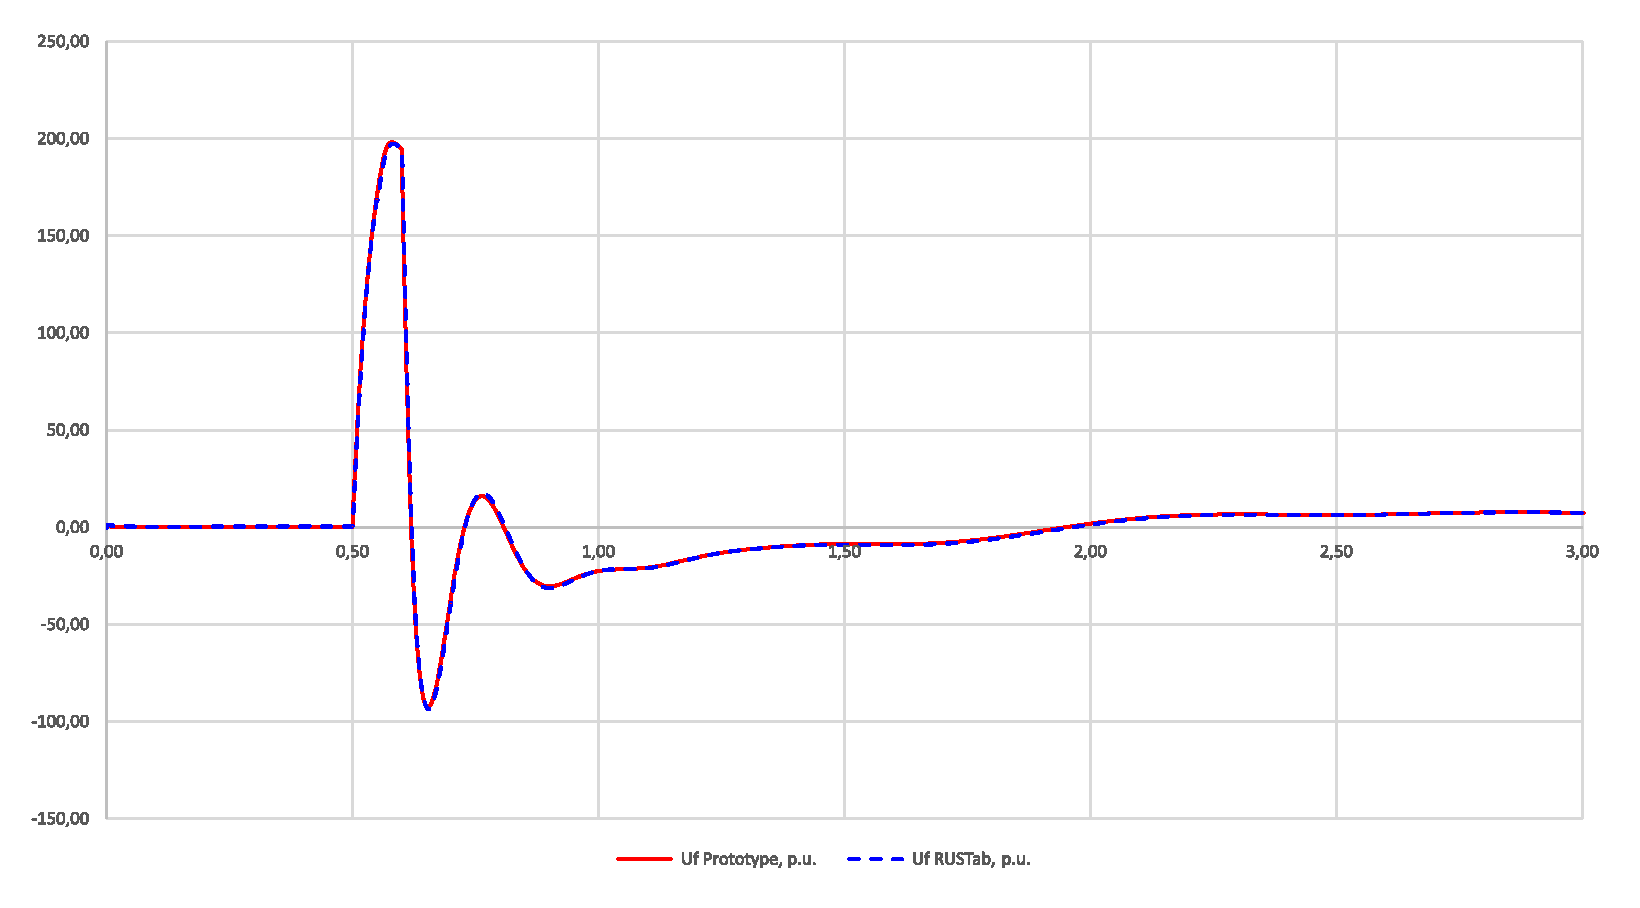
\includegraphics[width=\columnwidth]{case1state.eps}
	\caption{Comparison of simulation results of AVR outputs for case 1}
	\label{case1state}
\end{figure}

In the Fig. \ref{case1step} comparison of integration step sizes if shown. The Fig. \ref{case1stepz} shows zoomed version of the RUSTab step size to depict its step size control results. The implicit method allows much larger step sizes when transient decays due to its superior numerical stability.

\begin{figure}[htbp]
	\centering
	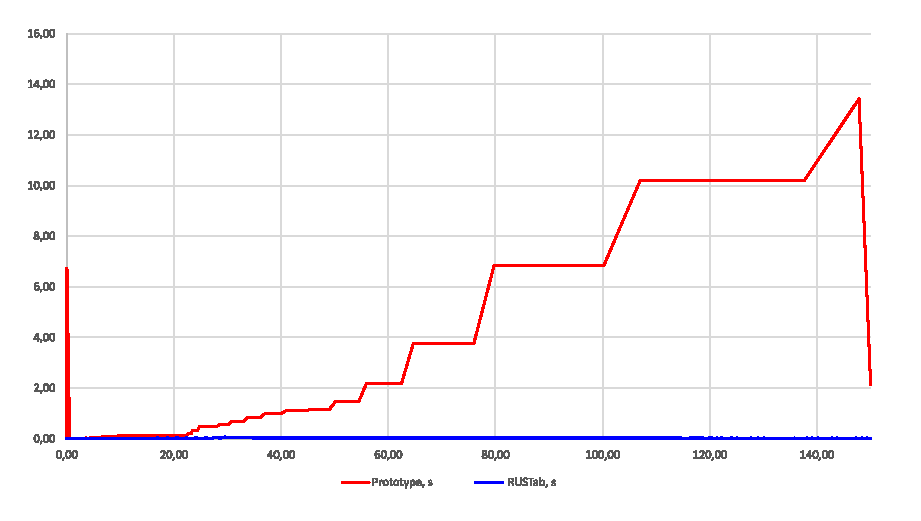
\includegraphics[width=\columnwidth]{case1step.eps}
	\caption{Comparison of integration steps for case 1}
	\label{case1step}
\end{figure}

\begin{figure}[htbp]
	\centering
	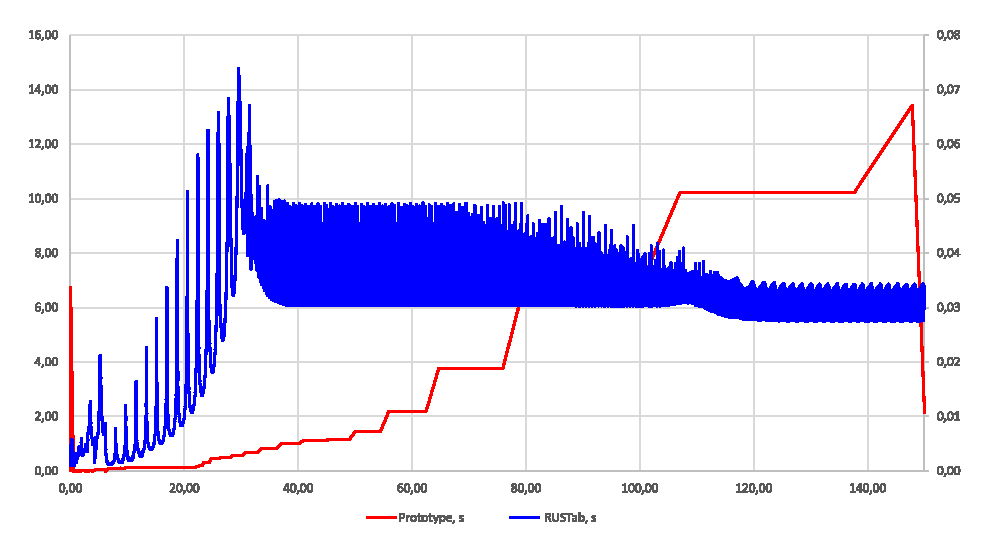
\includegraphics[width=\columnwidth]{case1stepz.eps}
	\caption{Comparison of integration steps for case 1 (zoomed)}
	\label{case1stepz}
\end{figure}

The times of simulations are shown in the Table \ref{tab:case1perf}.

\begin{table}[!h]
	\caption{Time of simulation and step count for the case 1\label{tab:case1perf}}
	\centering
	\begin{tabularx}{0.9\columnwidth}{ 
			| >{\raggedright\arraybackslash}X 
			| >{\raggedleft\arraybackslash}X 
			| >{\raggedleft\arraybackslash}X  
  	 	    | >{\raggedleft\arraybackslash}X |}
		\hline
 		 & \multicolumn{1}{c|} {RUSTab \(10^{-5}\)} & \multicolumn{1}{c|} {Prot. \(10^{-4}\)} & \multicolumn{1}{c|} {Prot. \(10^{-2}\)}\\ 
		\hlineB{3}	
		Time, s  & 77.9 & 4.0 & 3.7\\
		\hline
		Steps & 10628 & 2503 & 1842 \\
		\hline
	\end{tabularx}
\end{table}


\begin{figure}[htbp]
	\centering
	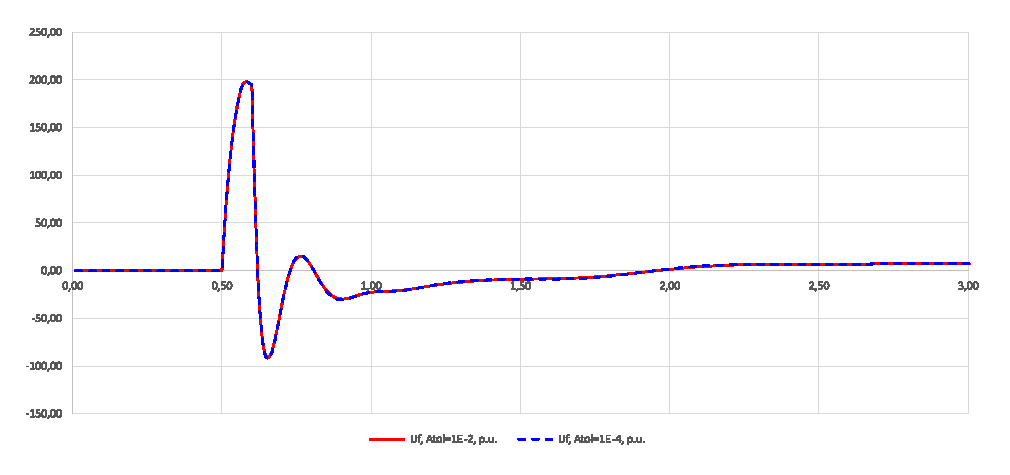
\includegraphics[width=\columnwidth]{case1atols.eps}
	\caption{Comparison of simulation results with different tolerances for case 1}
	\label{case1atols}
\end{figure}

\begin{figure}[htbp]
	\centering
	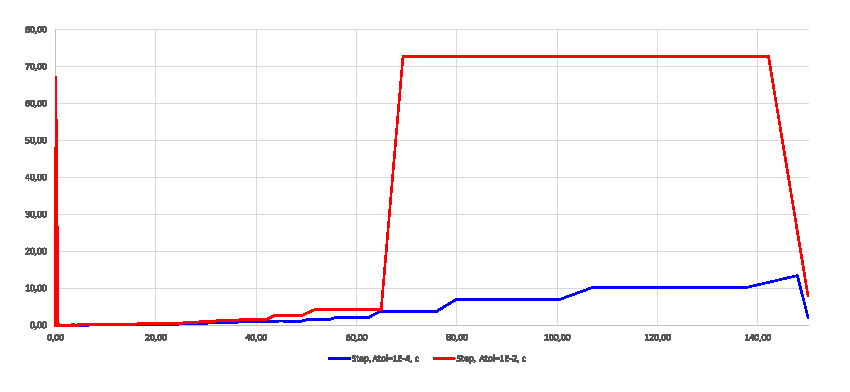
\includegraphics[width=\columnwidth]{case1atolsstep.eps}
	\caption{Comparison of integration step sizes with different tolerances for case 1}
	\label{case1atols}
\end{figure}


\begin{figure}[htbp]
	\centering
	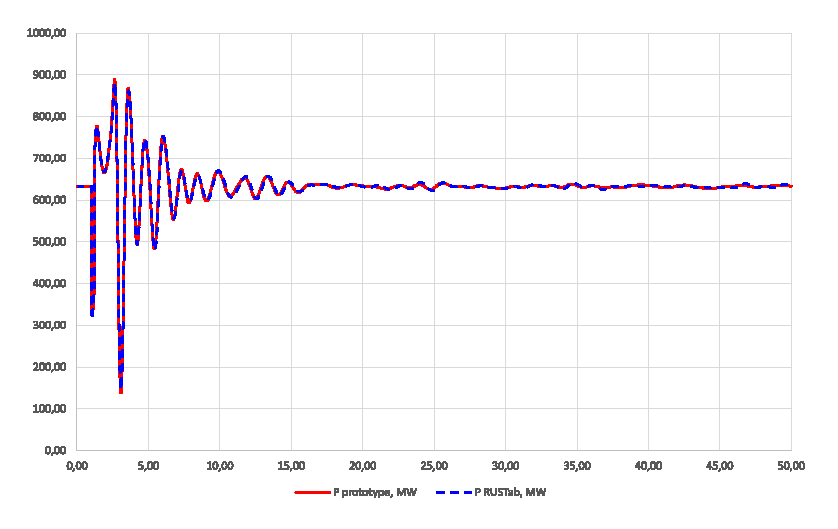
\includegraphics[width=\columnwidth]{case2state.eps}
	\caption{Comparison of simulation results of the generator output for case 2}
	\label{case2state}
\end{figure}

\begin{figure}[htbp]
	\centering
	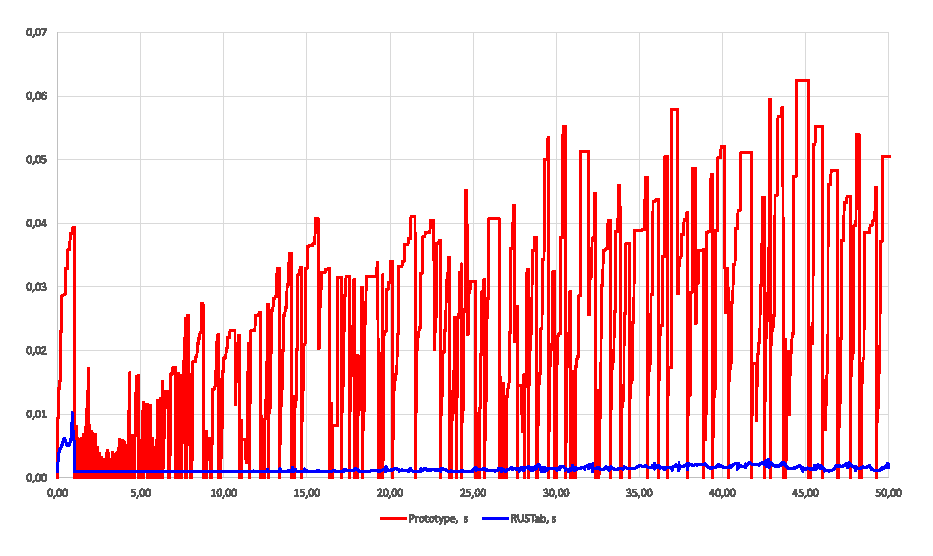
\includegraphics[width=\columnwidth]{case2step.eps}
	\caption{Comparison of integration steps for case 2}
	\label{case2step}
\end{figure}


\begin{figure}[htbp]
	\centering
	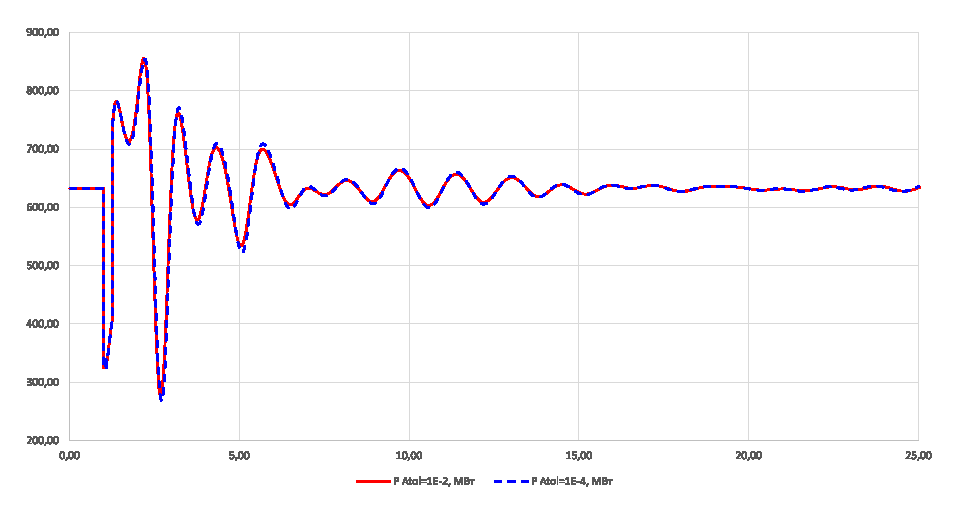
\includegraphics[width=\columnwidth]{case2atols.eps}
	\caption{Comparison of simulation results with different tolerances for case 2}
	\label{case2atols}
\end{figure}

\begin{figure}[htbp]
	\centering
	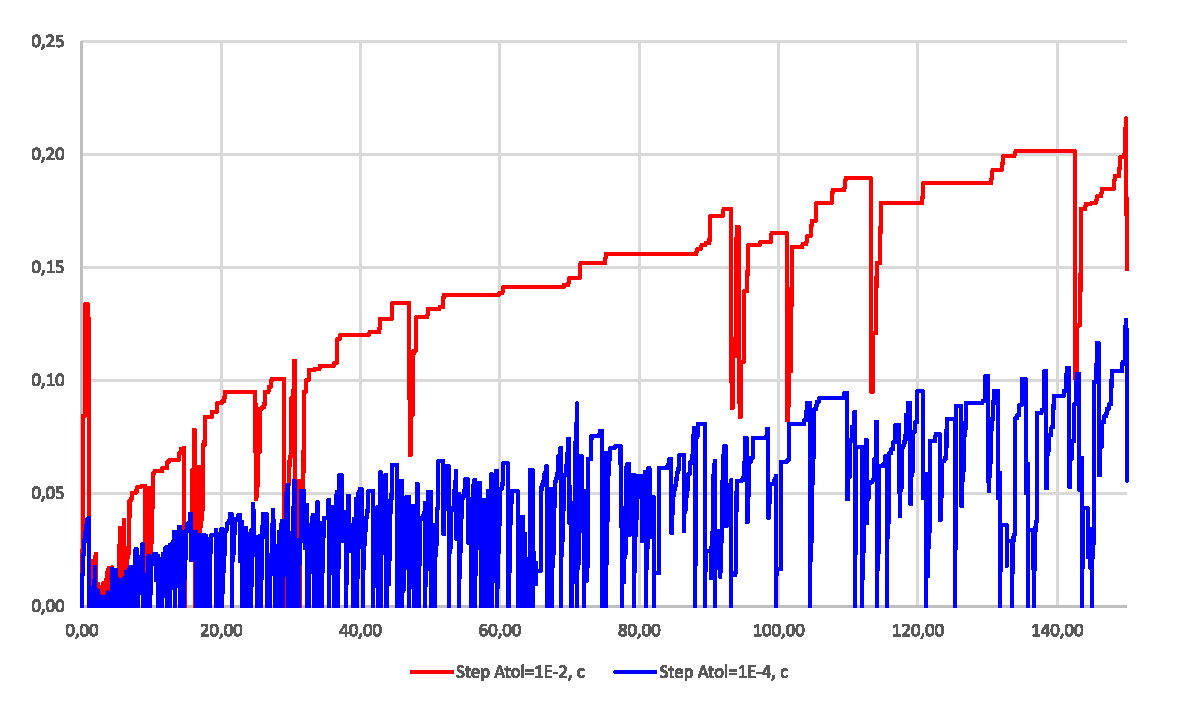
\includegraphics[width=\columnwidth]{case2atolsstep.eps}
	\caption{Comparison of integration step sizes with different tolerances for case 2}
	\label{case2atols}
\end{figure}

\begin{table}[!h]
	\caption{Time of simulation and step count for the case 2\label{tab:case2perf}}
	\centering
	\begin{tabularx}{0.9\columnwidth}{ 
			| >{\raggedright\arraybackslash}X 
			| >{\raggedleft\arraybackslash}X 
			| >{\raggedleft\arraybackslash}X  
			| >{\raggedleft\arraybackslash}X |}
		\hline
		& \multicolumn{1}{c|} {RUSTab \(10^{-5}\)} & \multicolumn{1}{c|} {Prot. \(10^{-4}\)} & \multicolumn{1}{c|} {Prot. \(10^{-2}\)}\\ 
		\hlineB{3}	
		Time, s  & 4685.6 & 279.1 & 98.6\\
		\hline
		Steps & 79395 & 11293 & 3909 \\
		\hline
	\end{tabularx}
\end{table}


\bibliographystyle{IEEEtran}
\bibliography{raiden}


%\newpage
\section{Biography Section}
\vspace{-33pt}
\begin{IEEEbiography}[{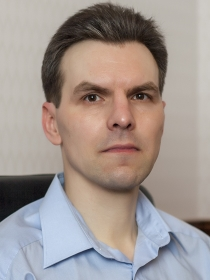
\includegraphics[width=1in,height=1.25in,clip,keepaspectratio]{mashalov}}]{Eugene Mashalov}
Graduated from Electrotechnical Faculty, Ekaterinburg, Urals State Polytechnical University, 1997. 
Received Ph.D degree in 2000 from the same university. 
Works for JSC "Scientific and Technical Center of Unified Power System", Ekaterinburg, Russia.\\
mashalov@gmail.com \\
www.inorxl.com
\end{IEEEbiography}
\vfill
\end{document}


